\section{Problem}\label{sec:problemdef}

\subsection{Problem setting}\label{subsec:probset}
We assume a setting where owners of mobile, positioning enabled, devices want route planning assistance. We assume users prefer online route planning services over offline solutions. 
We expect users to use network enabled capable of determining and visualizing users location and route.
Users want fast response times from online services, comparable to using an offline application \cite{ref}
Using a cache reduces the computational burden \cite{ref} on an online service, providing faster end-user response time \cite{ref} by both freeing up computational resources to calculate \spath routes, as well as being able to immediately provide the \spath result from the cache.
We consider only server side caching..



\subsection{Architecture}

The system architecture of what we propose is shown in fig. \ref{fig:advancedroutequery}B. 


\begin{figure}
  \center
	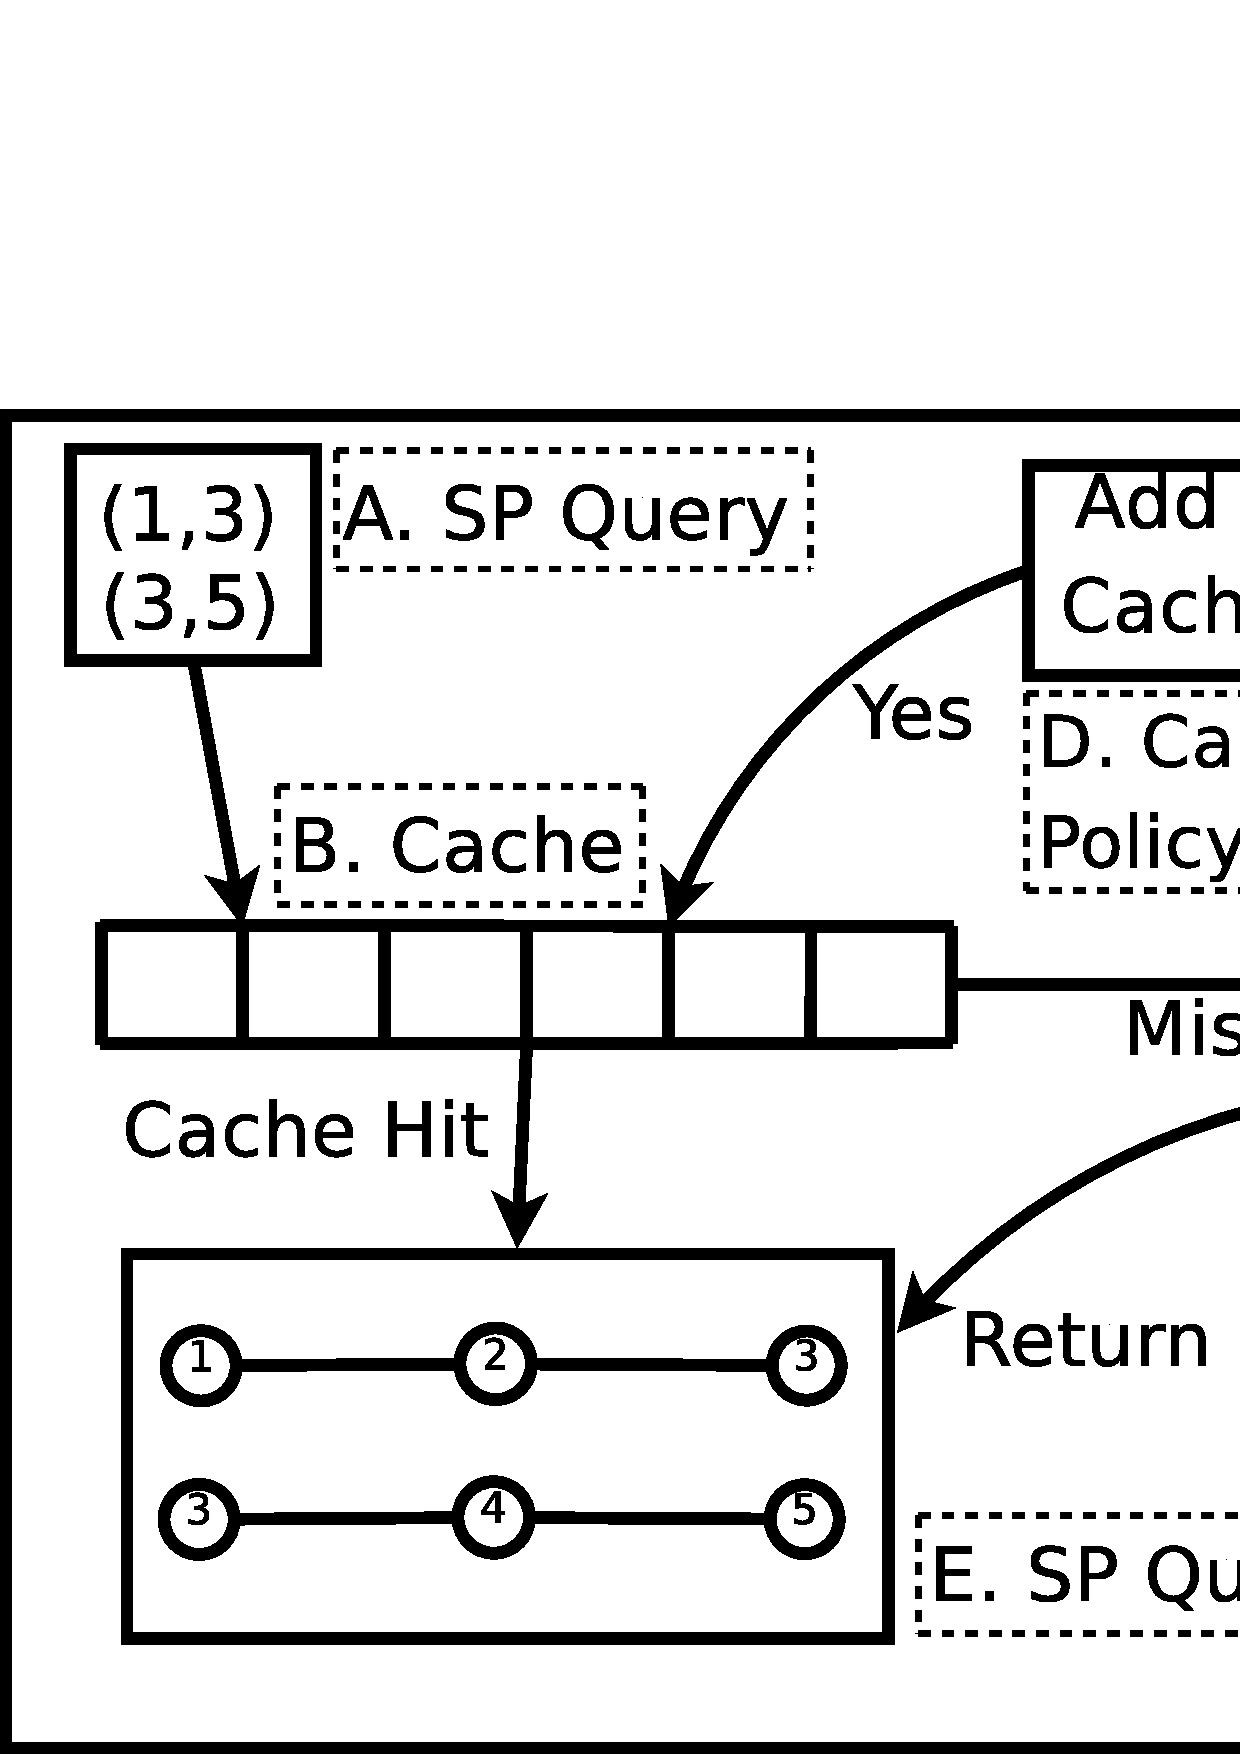
\includegraphics[width=0.55\textwidth]{figures/advancedroutequery.pdf}
	\caption{Advanced graph}
  \label{fig:advancedroutequery}
\end{figure}

\begin{table}
\begin{tabular*}{\columnwidth}{|l||p{0.77\columnwidth}|}
\hline
Symbol		& Meaning \\\hline
\spath		& Shortest Path \\\hline
LRU		& Least Recently Used \\\hline
FIFO		& First In First Out \\\hline
OSC		& Set of edges \\\hline
\acs{SPS} 	& \acl{SPS} \\\hline
\end{tabular*}
\caption{Table of symbols and notation} 
\label{tab:symbols}
\end{table}


To enable us to better argue about the real performance, as well as the strong and weak points of our ideas, we use a gaussian distribution model for the queries together with a graph with 6100/7035 vertices/edges.

\ffh{add about text: space per edge} 

\subsection{Optimization goals}\label{subsec:goals}

The overall goal, and most important measuring point to evaluate our success, is the reduction in CPU time (execution time) used compared to the same workload without any cache or optimizations.

At any \spath service provider the CPU time needed is roughly divided into the execution of the \spath algorithm and overhead related to query processing and system maintenance. 

We will be working on optimizing two sub-goals:
\begin{enumerate}
\item \label{it:sptime} Reducing the total time executing the \spath algorithm.
\item \label{it:ovtime} Reducing the total time spent on overhead.
\end{enumerate}


As stated in sub-goal \ref{it:sptime} we want to reduce reduce the time spent executing the \spath algorithm. We choose this goal as the \spath algorithm is usually the single most CPU intensive task at a \spath service \cite{ref.} and by using a cache we should be able to find a direct correspondence between cache hits and the total CPU time of the \spath algorithm.

In a \spath service without a cache there should a small amount of overhead related mainly to handling the incoming queries and system maintenance. Sub-goal \ref{it:ovtime} is about reducing this overhead. We want to reduce the overhead as adding a cache to a \spath system may add more overhead related to maintaining the cache integrity.

It is important that the increase in overhead does not grow larger than savings archived from the reduced time the \spath algorithm needs to be run.



% \section{Problem setting}\label{sec:problemdef}
% 
% We introduce relevant notations, define system requirements and specify
% the behavior of the proposed service. 
% 
% 
% First we briefly summarize the general scenario again. We assume users are willing to upload the positioning data from the routes (trajectories) they take when they move around on a road network. The system then anonymizes the trajectories according to a user specified "Privacy Profile" (Sec.~\ref{sec:usrprofile}), specifying which places or routes are sensitive to the user (Fig.~\ref{fig:overview}A, 1-5). After anonymization the system makes the data available to potential service providers for whom it guaranties a minimum level of data quality.
% 
% 
% \subsection{Problem Definition}\label{subsec:probdef}
% 
% \begin{table}
% %\begin{tabular*}{0.8\columnwidth}{|p{0.2\columnwidth}|l|p{0.25\columnwidth}|}
% \begin{tabular*}{\columnwidth}{|l||p{0.77\columnwidth}|}
% \hline
% Symbol		& Meaning \\\hline
% MD		& Mobile Device \\\hline
% $\mathbf{U}$	& Set of MDs \\\hline
% $\mathbf{V}$	& Set of vertices \\\hline
% $\mathbf{E}$	& Set of edges \\\hline
% $G(\mathbf{V,E})$ & Road network \\\hline
% $\mathbf{P}$	& Collection of all PSRs \\\hline
% $\mathbf{T}$	& Set of trajectories \\\hline
% $\Gamma$	& Set of all trajectories which contains sensitive PSR $p$ \\\hline
% RT		& Road Type \\\hline
% AS		& Protection scheme: Always Sensitive \\\hline
% ASTI		& Protection scheme: Always Sensitive with time interval \\\hline
% RS		& Protection scheme: Rarely sensitive \\\hline
% 
% \end{tabular*}
% \caption{Table of symbols and notation} 
% \label{tab:symbols}
% \end{table}
% 
% 
% We assume a setting where all users are equipped with a \md able to communicate and report
% the users position. All  \mds are online and are continuesly reporting the users location at
% predefined intervals. We use the terms {\it user, mobile device, and client} interchangeable and 
% denote the set of \mds by  $\mathbf{U} \subset \mathbb{N}$. We expect a \md to be cabable of visualizing its current location.
% 
% We assume a 2D scenario, where the movements of users $u \in \mathbf{U}$ are restricted to a road network $G(\mathbf{V,E})$.
% $\mathbf{V}$ is the set of vertices, where each vertex $v \in \mathbf{V}$ represents either a street intersection or an important landmark. $\mathbf{E}$ is the set of directed edges augmented by edge length and type. Edges are represented by a begin/end vertex pair and each edge represents the smallest unit of a road segment. $e \in \mathbf{E}$, each $e$ being a tuple specifying id, start-/end-vertices, length, and \rt $(e_{id},v_s,v_e,e_{length},e_{RT})$. \rt is a hierarchy of the size/type of road i.e. highway, paved, or dirt road (Sec.~\ref{subsec:roadtypes}).
% 
% The simplest form of trajectory is a collection of tuples $(time,longitude,latitude)$, ordered by the time attribute, but as we will work on a road network and in the spatio-temporal domain, such a basic notion of trajectories is not appropriate. 
% We define $\mathbf{T}$ as the set of trajectories, where each trajectory consist of an id $(t_{id})$, and a sequence of tuples containing an edge and start-/end-time ($\tau_{s_i}/\tau_{e_i}$) of edge traversal. A trajectory is then  $(t_{id}, \langle (e_{_j},\tau_{s_j},\tau_{e_j}), \ldots,(e_{_k}, \tau_{s_k},\tau_{e_k}) \rangle)$, where $t_{id}  \in \mathbb{N}$, $\tau_{s_i},\tau_{e_i}  | \tau_{s_i} < \tau_{e_i} \wedge \tau_{s_{i-1}} < \tau_{s_{i}} \wedge \tau_{e_{i-1}} < \tau_{e_{i}}, \tau_{s_i} \in \mathbb{N}, \tau_{e_i} \in \mathbb{N}$, and $e \in \mathbf{E}$, the set of edges. We restrict trajectories to the road network, and users are assumed to traverse the entirety of an edge.
% 
% A user $u \in \mathbf{U}$ is defined by a tuple $(u_{id}, \{s\}, \{t\})$, $u_{id} \in \mathbb{N}$, $s \in \mathbf{S}$ the set of Privacy Profiles (Sec.~\ref{sec:usrprofile}), and $t \in \mathbf{T}$. 
% 
% Traditional ways of obtaining user privacy often include spacial obfuscation by including the user in a bounding box, or cloaking region \cite{trajecGeneral09, semantic08}. Conventional classification methods working on trajectories \cite{Li2007, outlier09, outlier08} are not suited to work on cloaking regions, and applying such anonymization techniques will break these algorithms or require them to be modified to still function correctly.
% 
% Our approach has identical input and output format and keep the format simple by just having a list of trajectory ids, each one associated with a list of edge ids and their start-/end traversal time. We will thus not require any modifications of the traditional approaches for them to work on the anonymized dataset. The input format chosen only require a map to have ids on road edges, a reasonable assumption of most map data.
% After anonymization road edges may have been removed, and timestamps may have been modified, the output format is however still identical to the input format.
% 
% $\{\forall u \in \mathbf{U}\}$ specify at least one privacy profile. Each privacy profile specify the privacy settings for each section of road, such that for an edge  $e \in \mathbf{E}$ traversed by the user, the system will anonymize $e$ according to the privacy profile of $u$. Users need only specify one privacy profile, but may have more to cover different user contexts, e.g. work week, weekend, vacation.
% 
% 
% We want to develop a solution for the described approach, accomplishing the following important goals:
% \begin{itemize}
% 	\item {\bf Usability }
% 		To be useful, the privacy requirements has to be simple for the user to define.
% 	\item {\bf Practical }
% 		Besides when user specify his privacy profile, it should not require user interaction while running correctly.
% 	\item {\bf Flexible }
% 		Handle users specifying specific sensitive locations as well as specifying "everything but this" is sensitive.
% \end{itemize}
% 
% 
% % The proposed approach must be computationally efficient and the anonymized dataset must still contain enough data that the following two types of data analysis can be performed %with $i$, where $i$ is the percentage of extra errors introduced for each type of analysis after anonymization has been performed.
% % \begin{itemize}
% % 	\item Which sub-trajectories are popular when traveling from point A to point B.
% % 	\item When and where does the road segments experience high load
% % \end{itemize}
% 
% Given a set of user $u \in \mathbf{U}$ with a set of privacy profiles $s \in \mathbf{S}$ and a set of trajectories $t \in \mathbf{T}$ on a road network $G(\mathbf{V,E})$ the problem is then for each $u$ to apply $s$ on $\{t\}$.